\documentclass[11pt]{article}
\usepackage[english,serbian]{babel}
\usepackage{graphicx}
\usepackage{epsfig}
\usepackage{subcaption}
\usepackage{hyperref}
\usepackage{color}
\usepackage{url}
\usepackage[T2A]{fontenc} % enable Cyrillic fonts
\usepackage[utf8]{inputenc}
\hypersetup{colorlinks,citecolor=green,filecolor=green,linkcolor=blue,urlcolor=blue}
\graphicspath{{/home/max/Pictures/Screenshots}}

\begin{document}

\title{Digitalni zvuk\\ \small{Seminarski rad u okviru kursa\\Tehničko i naučno pisanje\\ Matematički fakultet}}

\author{Dusan Zugic, Nina Ostojic....\\ kontakt email adresa autora}
\date{15.~novembar 2022.}
\maketitle

\abstract
Ovaj seminarski rad pokušava da na jedan pregledan i koncizan način predstavi opšti uvid u digitalni zvuk, počevši od samog pojma zvuka, kratkog istorijata snimanja, razlika između analognog i digitalnog signala, te ulazi malo detaljnije u proces digitalizacije (odabiranje, kvantizacija i kodiranje), sa osvrtom na snimanje, čuvanje, kompresiju i formate zvuka, da bi na kraju sve bilo zaokruženo podvlačenjem značaja digitalnog zvuka, ciljevima digitalizacije i kako to utiče na sveopštu kulturu i izmenjeno lice sveta.

\tableofcontents

\section{Digitalizacija zvuka}
Za razliku od analognog zvuka koji je neprekidni signal u vremenu, digitalni zvuk je isprekidan i postoji samo u određenim trenucima vremena. Digitalizacija se najviše koristi jer su informacije na analognim nosačima zvuka sklone oštećenju reprodukcijom. Za digitalizaciju je potreban računar sa zvučnom karticom i programom za obradu zvuka, zatim uređaji za reprodukciju koji se digitalizuju (gramofon, kasetofon itd.) Radi boljeg kvaliteta dobro je koristiti i dodatnu opremu kao miksetu i pretpojačalo. Digitalizovani zvuk se otprema u jednom od formata: MP3, WAV, AIFF, AAC, OGG i dr.

Da bi se zvuk iz analognog preveo u digitalni oblik potrebno je izvršiti \textit{uzorkovanje}, \textit{kvantizaciju} i \textit{kodiranje}.

\subsection{Odabiranje ili uzorkovanje, semplovanje (engl. \textit{sampling})}
Uzorkovanje je postupak kojim se uzima vrednost električnog napona signala u određenim trenucima vremena. Što je kvalitet signala bolji, informacija će biti bolje digitalizovana, što znači što je uzorkovanje veće, kvalitetniji će biti dobijeni zvuk. Frekvencija uzorkovanja treba da bude najmanje dva puta veća od najveće frekvencije analognog signala (Nikvist-Šenonova teorema odabiranja). Standardna frekvencija uzorkovanja je 44,1kHz, a može ići i do 192kHz. Opšte prihvaćen CD audio standard je 44.1kHz, DAT kasete (eng. \textit{Digital Audio Tape}) koriste frekvenciju od 48kHz, a zvukovi u igricama 11 ili 22kHz. Može se uzorkovati i na manjim frekvencijama, ali tada će se desiti gubici (na pr. na uzorkovanju od 1kHz dobijeni zvuk će biti neprepoznatljiv - slika~\ref{fig:slika1}). Međutim, što je frekvencija uzorkovanja veća, to je veći i zapis, tj. zauzima više mesta kod čuvanja.

\begin{figure}[h]
    \centering
    \begin{subfigure}[t]{0.49\textwidth}
        \centering
        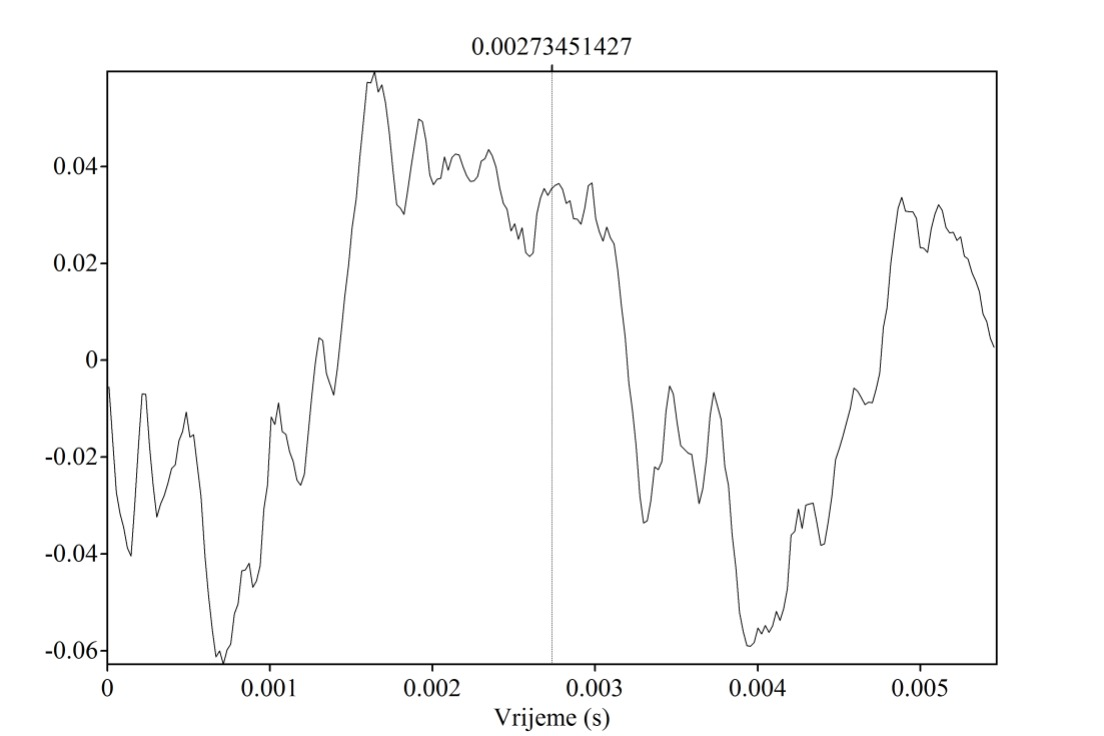
\includegraphics[width=1\textwidth]{Uzorkovanje1}
    \end{subfigure}
    \hfill
    \begin{subfigure}[t]{0.49\textwidth}
        \centering
        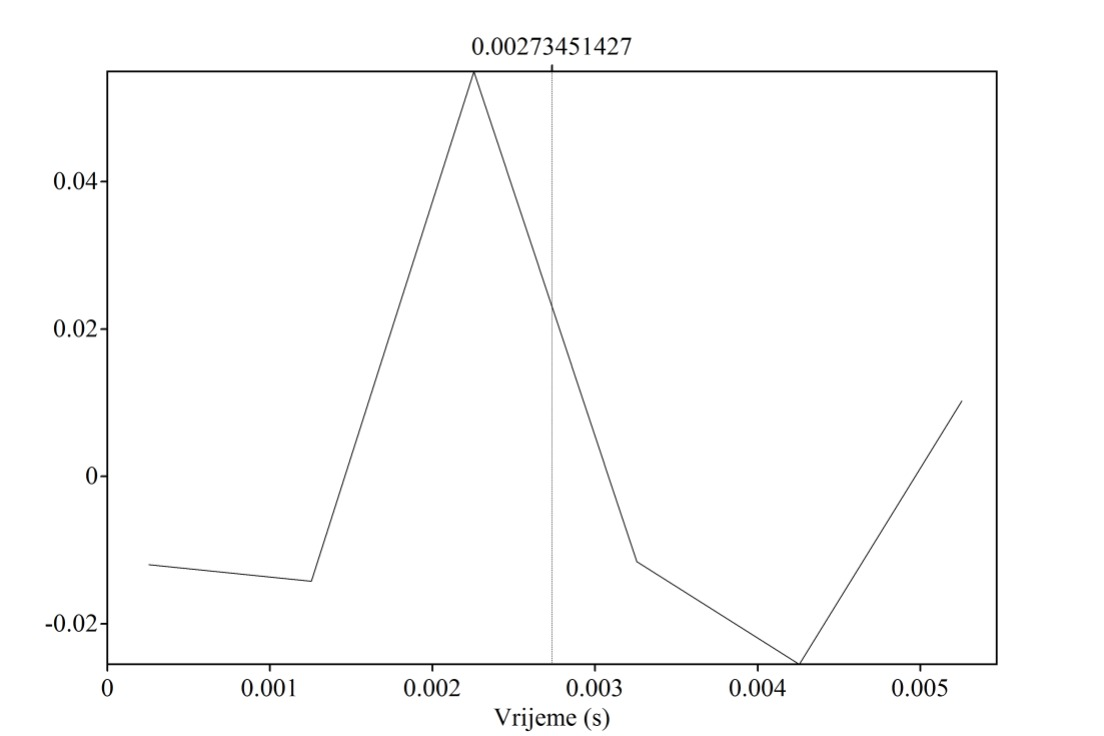
\includegraphics[width=1\textwidth]{Uzorkovanje2}
    \end{subfigure}
    \caption{Uzorkovanje na 44,1kHz i na 1kHz}
    \label{fig:slika1}
\end{figure}


\subsection{Kvantizacija}
Posle semplovanja ide kvantizacija što je postupak kojim se odabrane vrednosti električnog napona zaokružuju na najbližu od dozvoljenih vrednosti. Pošto jedna sekunda zvučnog zapisa može da se podeli na 44 100 delova (frekvencija uzorkovanja), svaki deo ima amplitudu koja nosi informaciju o zvuku, a ta informacija se prenosi u digitalni oblik, bit. Dubina bita se prikazuje formulom: 2x = n, gde je x broj bitova, a n broj mogućih kombinacija. Kvalitet zvuka direktno proporcionalno zavisi od broja bitova. Za digitalizaciju je standardan 16-bitni prikaz. Tokom kvantizacije neophodno dolazi do kvantizacijske greške (eng. \textit{quantization error}) koja uzrokuje šum u zapisu jer neminovno dolazi do gubitka informacije. Međutim, taj šum se obično ne primećuje.

\subsection{Kodiranje}
Kodiranje (eng. \textit{Encoding}) je niz znakova u digitalnom formatu koji se koriste za prenos i skladištenje. To je i proces pretvaranja podataka u neki drugi format i često se koristi za redukciju veličine audio datoteke. Pri kodiranju svaka vrednost se predstavlja logičkim nulama i jedinicama, tj. bitovima. Broj bitova (8, 16, 24...) određuje dinamički raspon jačine zvuka, što se izražava u decibelima. U digitalizaciji (prevođenju analognog u digitalni signal), kao što smo rekli, frekvencija uzorkovanja mora da bude najmanje dva puta veća od najveće frekvencije analognog signala i, zavisno od broja bitova, interval je podeljen na 2n nivoa, te se digitalni signal sastoji od blokova n bitova. Metode kodiranja koje se ovde koriste su:
\begin{itemize}
    \item \textit{Pulsna kod modulacija} (eng. \textit{Pulse code modulation, PCM}) – intervali su jednako raspoređeni
    \item \textit{Delta modulacija} (eng. \textit{Delta modulation, DM}) – uzorci se ne razlikuju mnogog i potrebno je manje bitova nego kod PCM
\end{itemize}
Digitalizacija se obavlja u analogno-digitalnom pretvaraču (eng. \textit{A/D converter}). Bitska brzina (eng. \textit{bit rate}) je broj bitova obrađenih u jedinici vremena, tj, u ovom slučaju, koliko je kilobita u sekundi potrebno za smeštanje zvuka (kpbs – eng. \textit{kilobit per second}).


\end{document}